\documentclass[14pt]{extbook}
\usepackage{multicol, enumerate, enumitem, hyperref, color, soul, setspace, parskip, fancyhdr} %General Packages
\usepackage{amssymb, amsthm, amsmath, bbm, latexsym, units, mathtools} %Math Packages
\everymath{\displaystyle} %All math in Display Style
% Packages with additional options
\usepackage[headsep=0.5cm,headheight=12pt, left=1 in,right= 1 in,top= 1 in,bottom= 1 in]{geometry}
\usepackage[usenames,dvipsnames]{xcolor}
\usepackage{dashrule}  % Package to use the command below to create lines between items
\newcommand{\litem}[1]{\item#1\hspace*{-1cm}\rule{\textwidth}{0.4pt}}
\pagestyle{fancy}
\lhead{Progress Quiz 9}
\chead{}
\rhead{Version B}
\lfoot{8590-6105}
\cfoot{}
\rfoot{Fall 2020}
\begin{document}

\begin{enumerate}
\litem{
Solve the equation below. Then, choose the interval that contains the solution.\[ -5(18x + 11) = -15(-14x -7) \]\begin{enumerate}[label=\Alph*.]
\item \( x \in [-1.07, -0.43] \)
\item \( x \in [0.11, 0.19] \)
\item \( x \in [-0.52, -0.21] \)
\item \( x \in [-0.23, 0.05] \)
\item \( \text{There are no real solutions.} \)

\end{enumerate} }
\litem{
Solve the linear equation below. Then, choose the interval that contains the solution.\[ \frac{-5x -6}{8} - \frac{5x -3}{3} = \frac{-9x -7}{5} \]\begin{enumerate}[label=\Alph*.]
\item \( x \in [2, 4.4] \)
\item \( x \in [0.1, 3.1] \)
\item \( x \in [-1.6, 0.4] \)
\item \( x \in [7.2, 9.2] \)
\item \( \text{There are no real solutions.} \)

\end{enumerate} }
\litem{
Solve the equation below. Then, choose the interval that contains the solution.\[ -11(15x -9) = -2(-5x + 18) \]\begin{enumerate}[label=\Alph*.]
\item \( x \in [0.38, 0.42] \)
\item \( x \in [-0.39, -0.31] \)
\item \( x \in [0.28, 0.4] \)
\item \( x \in [0.71, 0.84] \)
\item \( \text{There are no real solutions.} \)

\end{enumerate} }
\litem{
Write the equation of the line in the graph below in Standard form $Ax+By=C$. Then, choose the intervals that contain $A, B, \text{ and } C$.
\begin{center}
    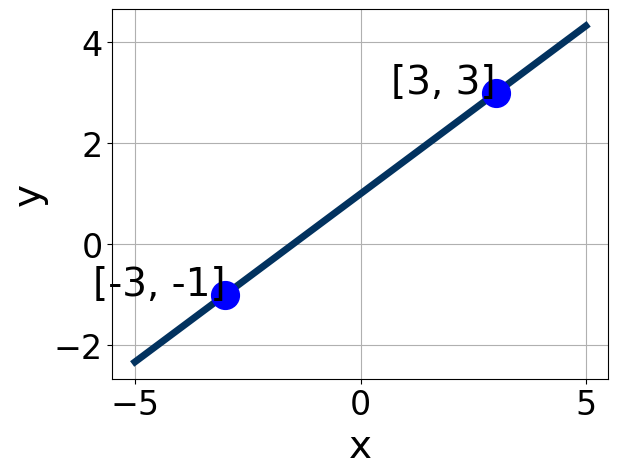
\includegraphics[width=0.5\textwidth]{../Figures/linearGraphToStandardCopyB.png}
\end{center}
\begin{enumerate}[label=\Alph*.]
\item \( A \in [-0.13, 1.46], \hspace{3mm} B \in [0.9, 3.2], \text{ and } \hspace{3mm} C \in [-5, -4] \)
\item \( A \in [1, 3.62], \hspace{3mm} B \in [3.5, 5.4], \text{ and } \hspace{3mm} C \in [-31, -23] \)
\item \( A \in [1, 3.62], \hspace{3mm} B \in [-7.8, -1.5], \text{ and } \hspace{3mm} C \in [23, 27] \)
\item \( A \in [-3.6, -1.74], \hspace{3mm} B \in [-7.8, -1.5], \text{ and } \hspace{3mm} C \in [23, 27] \)
\item \( A \in [-0.13, 1.46], \hspace{3mm} B \in [-4.7, 0.5], \text{ and } \hspace{3mm} C \in [5, 11] \)

\end{enumerate} }
\litem{
Solve the linear equation below. Then, choose the interval that contains the solution.\[ \frac{7x + 8}{4} - \frac{6x -4}{7} = \frac{7x + 4}{6} \]\begin{enumerate}[label=\Alph*.]
\item \( x \in [1.3, 2.9] \)
\item \( x \in [0.1, 1.1] \)
\item \( x \in [28.5, 30.9] \)
\item \( x \in [6.8, 7.5] \)
\item \( \text{There are no real solutions.} \)

\end{enumerate} }
\litem{
Find the equation of the line described below. Write the linear equation as $ y=mx+b $ and choose the intervals that contain $m$ and $b$.\[ \text{Perpendicular to } 7 x + 5 y = 14 \text{ and passing through the point } (-2, -5). \]\begin{enumerate}[label=\Alph*.]
\item \( m \in [0.71, 0.74] \hspace*{3mm} b \in [-3.55, -2.81] \)
\item \( m \in [0.71, 0.74] \hspace*{3mm} b \in [-4.18, -3.37] \)
\item \( m \in [0.71, 0.74] \hspace*{3mm} b \in [3.33, 3.91] \)
\item \( m \in [0.93, 1.67] \hspace*{3mm} b \in [-4.18, -3.37] \)
\item \( m \in [-1.51, -0.24] \hspace*{3mm} b \in [-6.55, -6.13] \)

\end{enumerate} }
\litem{
Find the equation of the line described below. Write the linear equation as $ y=mx+b $ and choose the intervals that contain $m$ and $b$.\[ \text{Parallel to } 3 x + 5 y = 13 \text{ and passing through the point } (-5, -10). \]\begin{enumerate}[label=\Alph*.]
\item \( m \in [-1.23, 0.45] \hspace*{3mm} b \in [-6.3, -3.9] \)
\item \( m \in [-1.23, 0.45] \hspace*{3mm} b \in [-13.4, -10.5] \)
\item \( m \in [-1.23, 0.45] \hspace*{3mm} b \in [11.9, 13.2] \)
\item \( m \in [-2.34, -0.92] \hspace*{3mm} b \in [-13.4, -10.5] \)
\item \( m \in [-0.37, 1.46] \hspace*{3mm} b \in [-8, -6.3] \)

\end{enumerate} }
\litem{
Write the equation of the line in the graph below in Standard form $Ax+By=C$. Then, choose the intervals that contain $A, B, \text{ and } C$.
\begin{center}
    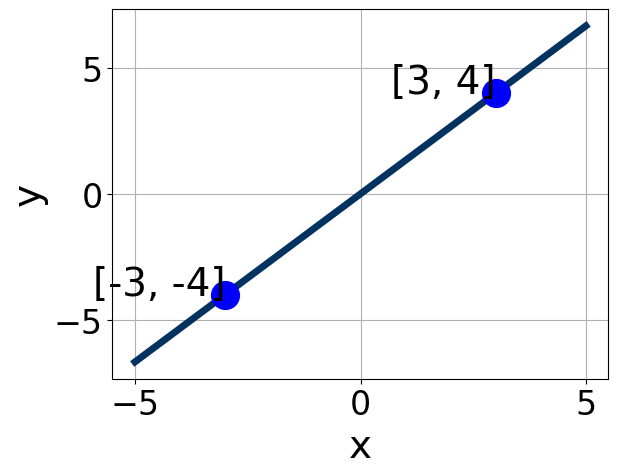
\includegraphics[width=0.5\textwidth]{../Figures/linearGraphToStandardB.png}
\end{center}
\begin{enumerate}[label=\Alph*.]
\item \( A \in [-4.8, 1.4], \hspace{3mm} B \in [0.46, 2.5], \text{ and } \hspace{3mm} C \in [-4, -1] \)
\item \( A \in [-5.9, -4.3], \hspace{3mm} B \in [2.76, 3.35], \text{ and } \hspace{3mm} C \in [-13, -6] \)
\item \( A \in [-4.8, 1.4], \hspace{3mm} B \in [-1.06, -0.45], \text{ and } \hspace{3mm} C \in [4, 10] \)
\item \( A \in [3.7, 6.9], \hspace{3mm} B \in [2.76, 3.35], \text{ and } \hspace{3mm} C \in [-13, -6] \)
\item \( A \in [3.7, 6.9], \hspace{3mm} B \in [-4.12, -2.96], \text{ and } \hspace{3mm} C \in [9, 13] \)

\end{enumerate} }
\litem{
First, find the equation of the line containing the two points below. Then, write the equation as $ y=mx+b $ and choose the intervals that contain $m$ and $b$.\[ (10, 5) \text{ and } (5, 9) \]\begin{enumerate}[label=\Alph*.]
\item \( m \in [-2.5, 0.7] \hspace*{3mm} b \in [12.6, 14.2] \)
\item \( m \in [-2.5, 0.7] \hspace*{3mm} b \in [-6.3, -2.6] \)
\item \( m \in [-2.5, 0.7] \hspace*{3mm} b \in [1.2, 4.2] \)
\item \( m \in [-0.1, 1.2] \hspace*{3mm} b \in [4.9, 5.9] \)
\item \( m \in [-2.5, 0.7] \hspace*{3mm} b \in [-13.4, -11] \)

\end{enumerate} }
\litem{
First, find the equation of the line containing the two points below. Then, write the equation as $ y=mx+b $ and choose the intervals that contain $m$ and $b$.\[ (-9, 4) \text{ and } (3, 2) \]\begin{enumerate}[label=\Alph*.]
\item \( m \in [-0.59, 0.03] \hspace*{3mm} b \in [-2.99, -2.1] \)
\item \( m \in [-0.07, 0.29] \hspace*{3mm} b \in [0.44, 1.9] \)
\item \( m \in [-0.59, 0.03] \hspace*{3mm} b \in [12.53, 13.34] \)
\item \( m \in [-0.59, 0.03] \hspace*{3mm} b \in [2.16, 2.59] \)
\item \( m \in [-0.59, 0.03] \hspace*{3mm} b \in [-1.57, -0.15] \)

\end{enumerate} }
\end{enumerate}

\end{document}